\documentclass{ximera}

\author{Anna Davis} \title{MTH 140 Homework 7} 

\begin{document}

\begin{abstract}

\end{abstract}
\maketitle
 \textit{Certificate due: 3/8/2021 at 11:59 p.m.}
 
 
 \begin{problem}\label{prob:140hom7extra1}
 Based on the data for 2015-17 graduates, the mean ACT Reading score was 21.4 with standard deviation of 6.5.  For each given ACT score, find an equivalent SAT score if SAT scores are approximately normally distributed with the distribution given by $X\sim N(1059,210)$.
 
 (Round your scores to the nearest integer.)
 
 An ACT score of 22 is equivalent to an SAT score of $\answer{1100}$.
 
 An ACT score of 19 is equivalent to an SAT score of $\answer{988}$.
 
 \end{problem}
 
  \begin{problem}\label{prob:140hom6prob2}
 Based on the data for 2015-17 graduates, the mean ACT Reading score was 21.4 with standard deviation of 6.5.  A sample of 100 Reading scores is chosen at random. 
 
 Summarize the given info:
$$\sigma=\answer{6.5}$$
$$\mu=\answer{21.4}$$
$$n=\answer{100}$$

\begin{center}  
\geogebra{emwxhga2}{800}{600}  
\end{center}
\begin{enumerate}
\item
What is the probability that the sample mean score is above 23?  (Use GeoGebra.  Enter your answer to four decimal places.)
$$\answer{0.0069}$$
\item What is the probability that the sample mean falls between 20 and 21?
$$\answer{0.2535}$$
\end{enumerate}
\end{problem}

\begin{problem}\label{prob:140hom6prob3}
The histogram below shows the distribution of average daily wind speeds measured at John Glenn International Airport in Columbus OH.
\begin{image}
   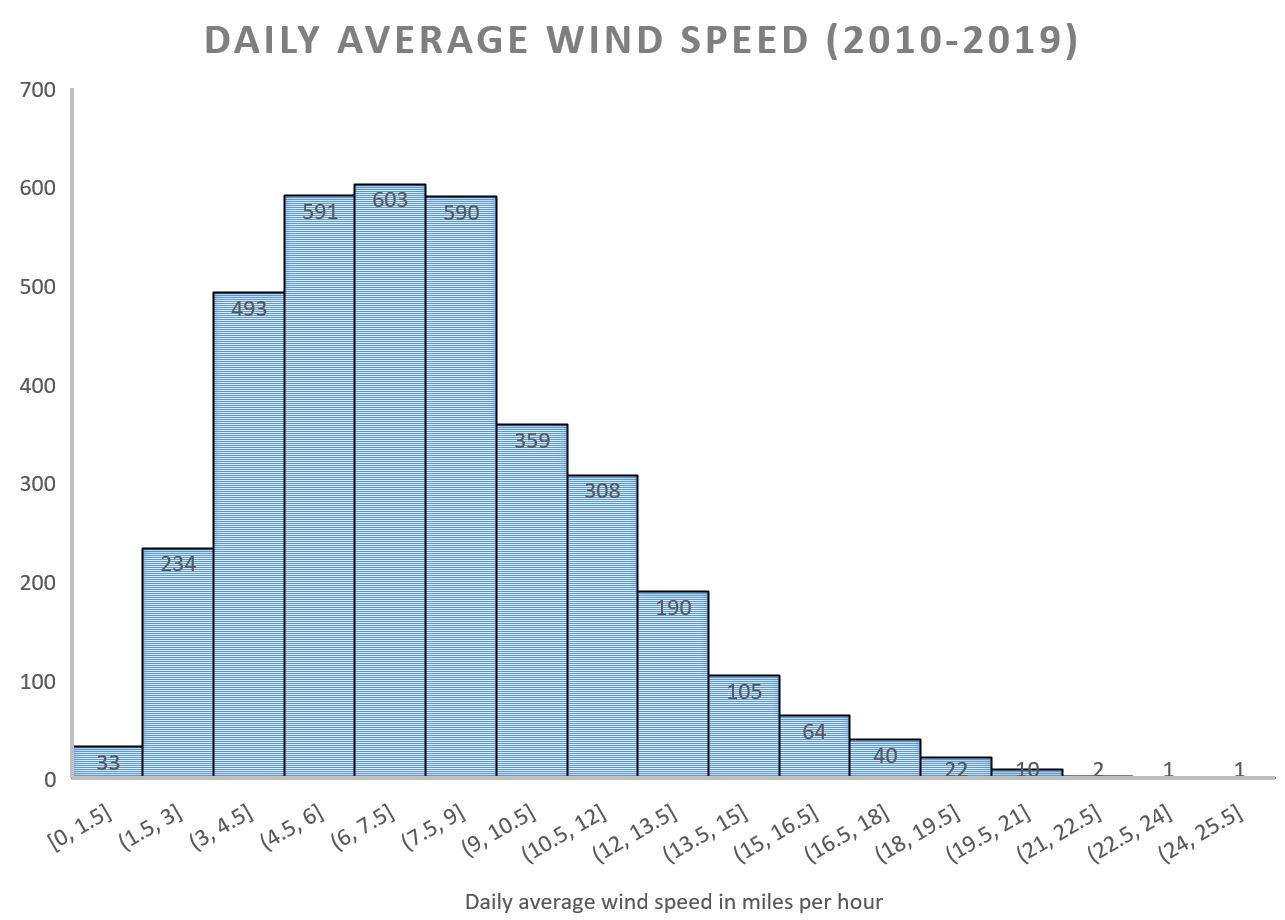
\includegraphics[height=1in]{140H6pic1.jpg}
 \end{image}
 The mean of the daily averages was found to be $\mu=7.6$ with standard deviation of $\sigma=3.6$.
 
 Answer each of the following questions using the Central Limit Theorem, IF POSSIBLE.  If the answer is impossible to find using the Central Limit Theorem, type NA into the answer box. (Case sensitive.)  Otherwise, use GeoGebra and enter your answers to four decimal places.
 \begin{enumerate}
     \item What is the probability that the average wind speed on a randomly chosen day is below 8 miles per hour?
     $$\answer{NA}$$
     \item What is the probability that a randomly selected sample of 36 days will yield a mean of less than 7.2?
     $$\answer{0.2525}$$
     \item What is the probability that the mean of daily averages for July of 2017 exceeds 8 miles per hour?
     $$\answer{NA}$$
     
 \end{enumerate}
\end{problem}
 



 
 \begin{problem}\label{prob:140hom6prob1}
 Based on meteorological daily data from the past ten years, the average of daily high temperatures in Columbus, OH is 63.7 degrees Fahrenheit, with standard deviation of 20.3 degrees. 
 
 According to the Central Limit Theorem...
     \begin{multipleChoice}  
\choice{It is possible to find the probability that five daily highs selected at random will have an average of above 65 degrees.}  
\choice{The standard deviation for the distribution of sample means for samples of size 10 is $\sigma_{\overline{x}}=\frac{20.3}{\sqrt{10}}$}  
\choice{If a sample of 60 consecutive days is chosen, the average temperature for the sample will be within 5 degrees of 63.7.}  
\choice{All of the above.}  
\choice[correct] {None of the above.}
\end{multipleChoice}

 \end{problem}
 
 
 
 
 
 
\end{document}